\nocite{*}
\chapter{Introduction}
\label{sec:introduction}

This section gives the reader a brief overview of the motivation, the context and the scope of this bachelor thesis.

\section{Motivation}

\textsc{Scubo} is a submersible robot (see Figure ~\ref{pics:scubo_robot}) developed in the scope of a focus project at ETH Zurich. During two semester, a team consisting of mechanical and electrical engineering students had the opportunity to build a functional prototype of a robot. The goal of the project was to design a manually controlled submersible robot which is capable for 3D reconstruction of single corals. By taking pictures from different sides and angles of the underwater object, a detailed model can be obtained in post-processing by feeding these pictures to a suitable third party software like \textsc{Pix4D}\footnote{https://pix4d.com/}. This way, changes of coral reefs can be well observed and documented. Furthermore, the robot should provide telepresence for exploration of underwater landscapes. With the help of six on-board cameras, the user has access to a visual feedback from all sides of the robot through a VR-headset. The overall goal for the future is a further development of \textsc{Scubo} into a fully autonomous system. This has the following benefits:  

\begin{itemize}
	\item 
	Common image processing software is based on finding keypoints\footnote{Characteristic points detected in an image.} between images, which will generate 3D points. By increasing the overlap between two images, the common area captured is larger and more keypoints can be detected and matched together. Consequently, a rule of thumb is to maintain high overlap between the images. This can be done by keeping a constant distance while slightly varying the angle to the object. Therefore, scanning corals via remote control is difficult since the user has to control the distance as well as the orientation of the robot to the object. This task can be simplified by generating an efficient trajectory consisting of position and orientation information around that object for the autonomous system to follow.
	\item 
	One possible application of \textsc{Scubo} and its virtual reality feature is the deployment in large aquariums of entertainment parks. These are narrow environments containing static as well as dynamic obstacles such as glass walls and underwater creatures. Collision in such sensitive surroundings would endanger the safety of the audience and the animals. This problem can be prevented by an autonomous system that is able to follow a predefined collision-free path. In this way, the audience can observe the environments through a VR-headset without having to control the robot. 
\end{itemize}

\begin{figure} [h]
	\centering
	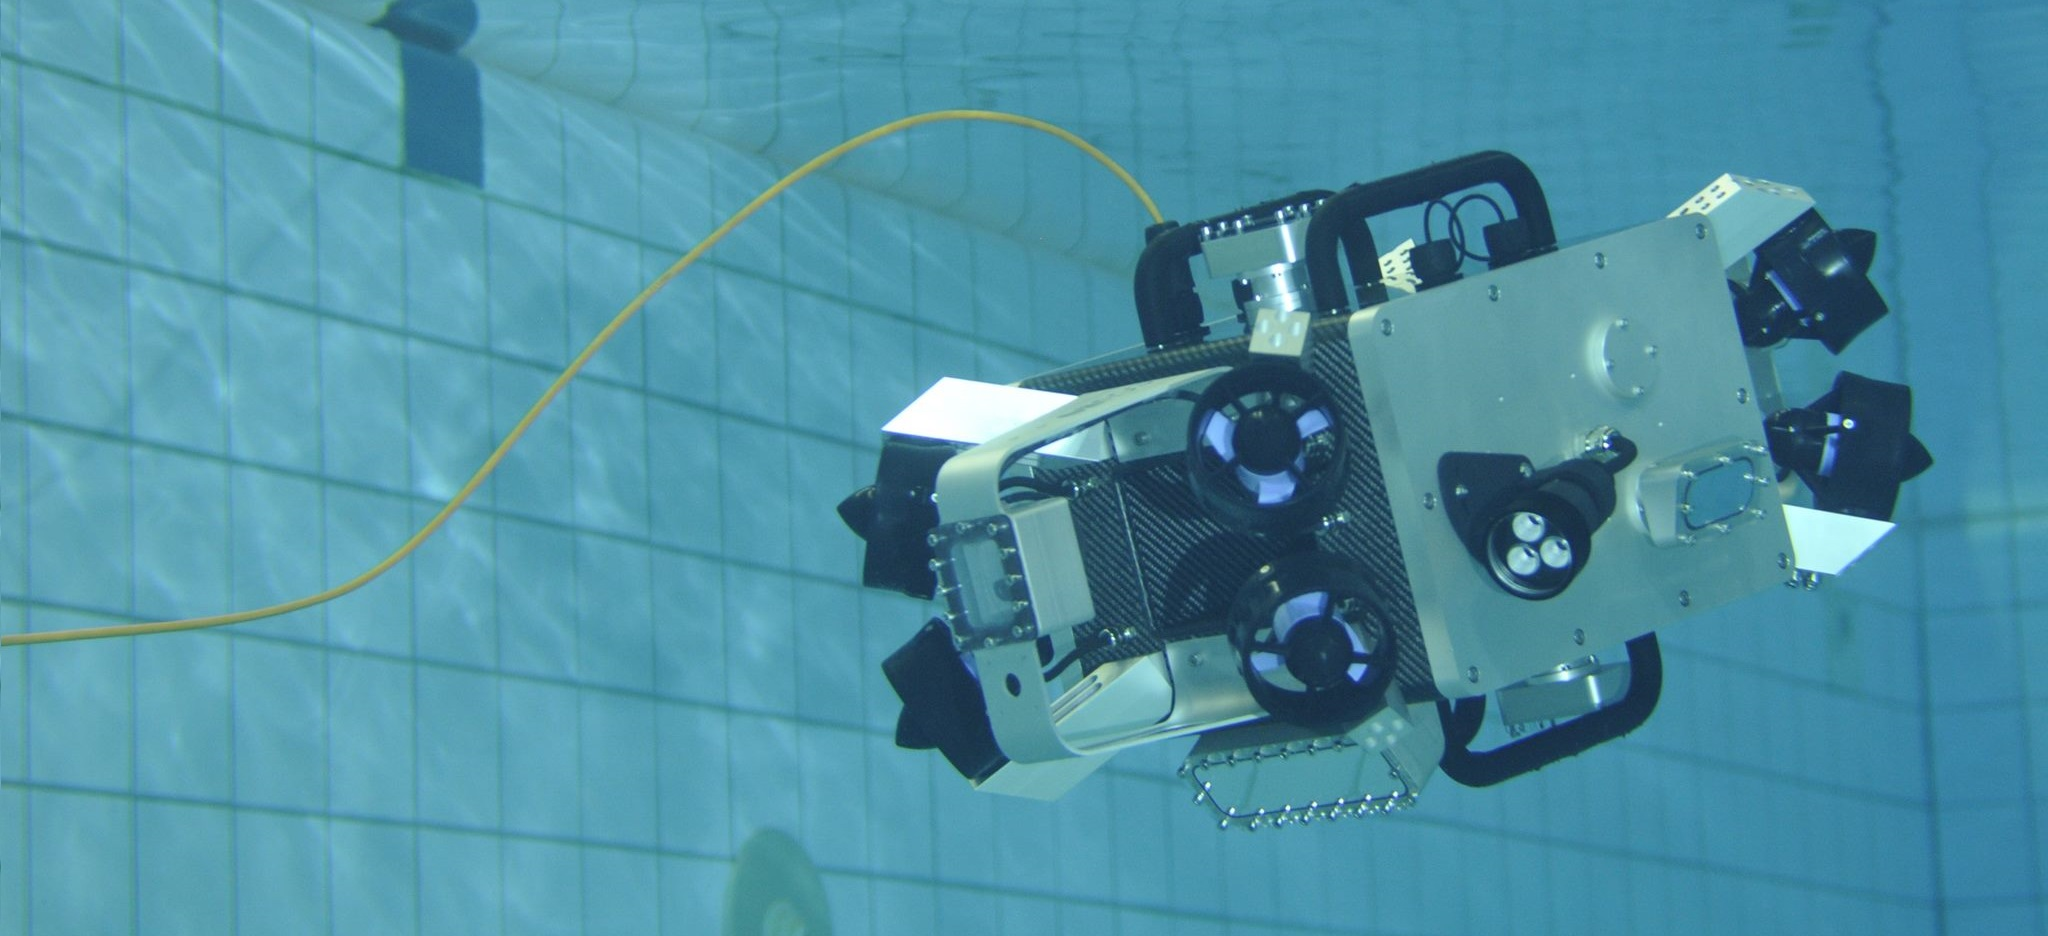
\includegraphics[width=0.9\textwidth]{images/Scubo_robot.jpg}
	\caption{The \textsc{Scubo} robot in action.}
	\label{pics:scubo_robot}
\end{figure}
  
\section{Context}  
  
This bachelor thesis discusses planning algorithm and aims to complement the work of the focus project \textsc{Scubo}. Together with several other bachelor theses, its goal is to build the foundation for an autonomous system based on computer vision. In the following an overview of the theses and their associations is given:

\begin{itemize}
	\item
	Underwater Camera Calibration: The process of determining all the necessary parameters for the image rectification in underwater application. 
	\item
	Localisation and Mapping: State estimation and 3D reconstruction of the environment to a point cloud by post-processing recordings of the calibrated stereo camera and an IMU (VIO-sensor). 
	\item
	Path Planning: Implementation of an algorithm which generates a collision-free trajectory from a starting to a destination point using the previous generated point cloud.
	\item 
	Trajectory Controller: Design of controller needed to follow the generated set of waypoints. 
\end{itemize}

\section{Goal}
The goal of this bachelor thesis is the development of an offline path planning algorithm as a basic for a semi-autonomous\footnote{The planning algorithm of a semi-autonomous system requires the complete map in advance and does not calculate the set of waypoints in real-time.} system. The designed algorithm should provide a set of global waypoints of position informations from start to finish while avoiding collision with obstacles. Furthermore, a method should be found to generate a trajectory around an object for scanning purpose. The following framework conditions apply: 

\begin{itemize}
	\item
	The visible areas by the robot is represented by a certain space called the workspace. The robot itself is represented in the workspace by its centre of mass point.  
	\item
	Obstacles in the form of a point cloud represents not accessible states.
	\item
	Starting and goal state are predefined input variables.	
\end{itemize}

	
